\subsection{Upgrade Design of the Protocol Code}
% \subsection{核心协议的升级设计}

We first give the block structure of the Nebulas, and then discuss how to upgrade the protocol code based on the block structure.

%我们首先给出星云链中的区块结构,然后讨论如何在该区块结构上实现核心协议的升级问题。

\subsubsection{Block Structure}

The Nebulas block data structure contains, but is not limited to, the following:

% 星云链区块数据结构包含,但不限于以下信息:
\begin{itemize}
	\item Header:Block Header
		\begin{itemize}
		\item Height:block height
		\item ParentHash:parent block hash
		\item Ts:timestamp
		\item Miner:miner address
		\item Dynasty:the consensus dynasty of the block
		\item Epoch:the consensus age of the block
		\item StateRoot:state root hash
		\item TxsRoot:transaction root hash
		\item ReceiptsRoot:transaction receipt hash
		\item TransNum:number of transactions
		\end{itemize}
	\item Transactions:transaction data (including multiple transactions)
		\begin{itemize}
		\item From:transaction sender address
		\item To:transaction receiver address, for creating a smart contract with a value 0x0
		\item Value:transfer amount
		\item Data:Transaction payload. It's the smart contract bytecode if the transaction is for creating a smart contract; It's the name of the calling function and the entry if the transaction is a smart contract call.
		\item Signature:transaction signature
		\item Gas:gas limit
		\item GasPrice:gas unit price
		\item Nonce:the uniqueness of transactions
		\end{itemize}
	\item Votes:Prepare and Commit Votes (including multiple), used in PoD (see \refsec{sec:pod}) consensus algorithm
		\begin{itemize}
		\item From:voter
		\item VoteHash:hash of the block voted for
		\item Hv:the height of the block voted for
		\item Hvs:the height of an ancestral block of the block voted for
		\item VoteType:voting type,Prepare or Commit
		\item Signature:vote signature
		\end{itemize}
	\item Protocol Code:The protocol code (only 0 or 1 in a block)
		\begin{itemize}
		\item Hash:hash of the protocol code
		\item Code:the bytecode of the protocol code
		\item ValidStartBlock:the start block number that protocol come into effect
		\item Signature:signautre (sign by the developer community)
		\item Version:the protocol code version number, and each upgrade needs to be incremented to prevent malicious accounts from rolling back to the old protocol code
		\item Nonce:the uniqueness of protocol code
		\end{itemize}
	\item Nebulas Rank:Nebula index (calculated once a week, most blocks haven't this section)
		\begin{itemize}
		\item RankVersion:NR version
		\item RankRoot:NR rank hash
		\item RankRecords:NR rank record
			\begin{itemize}
				\item Address:Account address tag
				\item Score:NR value
			\end{itemize}
		\end{itemize}
\end{itemize}

\begin{figure}[!h]
\centering
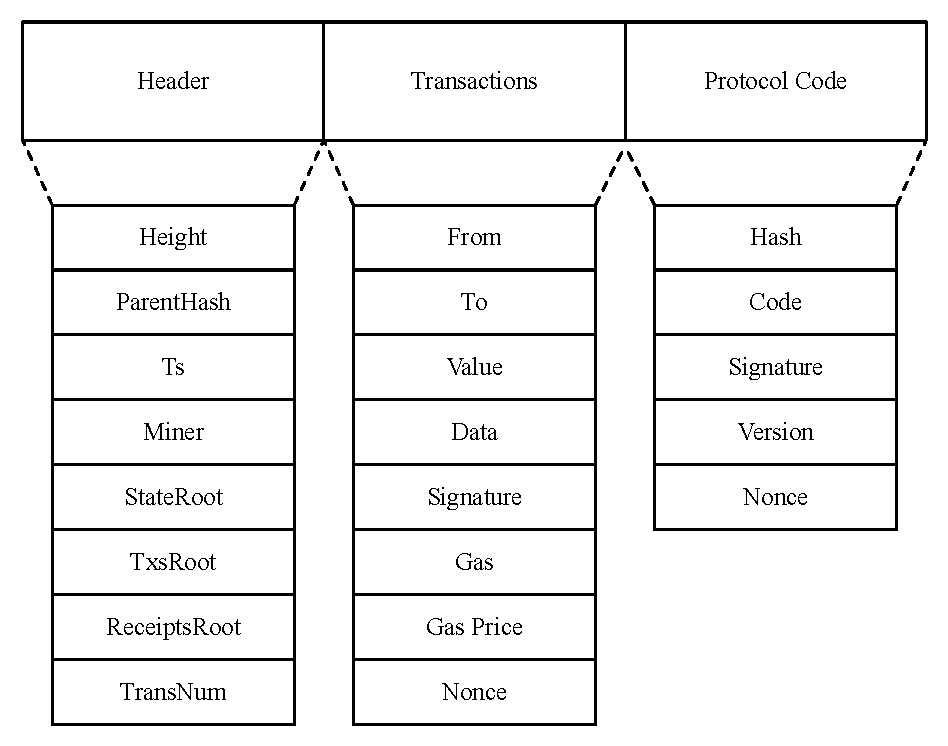
\includegraphics[width=13.8cm]{./figs/block}
\caption{Block Structure}
\label{fig:block}
\end{figure}

Similar to other cryptocurrency systems, the interaction between the account and the blockchain is done through a particular transaction. The account creates a transaction, which is signed with a private key, and sends it to any node in the blockchain and broadcasts it to full network node through the P2P network. During the fixed block time interval, the nodes specified by the PoD consensus algorithm (see \refsec{sec:pod}) collect all transactions in the time and pack them into blocks of standard format and broadcast them to the rest of the network. After verification by each node, the new block is appended into the local ledger and becomes a part of the global ledger.

%类似于其他加密数字货币系统,用户和区块链上的互动都是通过特定的交易进行的。用户创建一笔交易,用自己的私钥签名后,发到区块链的任何一个节点中,通过P2P网络广播到全网节点。在固定的出块时间间隔内,由PoD共识算法(见\refsec{sec:pod})指定的记账节点累计这段时间内的所有交易,打包成标准格式的区块,同步到全网所有节点。经各节点独立验证后,加入本地账本,成为全球总账本的一部分。

In Ethereum, transactions are divided into two types: ordinary account transaction and smart contract transaction. We add new transaction types to the blocks of Nebulas: protocol code and the Nebulas Rank. The protocol code, as a part of the blockchain data, is stored on the chain, and the upgrade of the basic protocol of Nebulas is carried out through supplementing additional data on chains. Based on the NR ranking algorithm, the NR value of each account is calculated in each cycle and saved in the corresponding chain to facilitate the real-time NR value calling and historical ranking query.

%以太坊中,交易分为两种类型:普通账户交易,智能合约交易。我们在星云链的区块中,增加新的数据类型:核心协议代码和星云指数。核心协议代码作为区块链数据的一部分存储在链上,星云链基础协议的升级,是通过链上数据的追加而实现的。星云指数根据NR排名算法,计算出每个周期各个账户的NR值存到链上,方便NR值的实时调用和历史排名查询。

\subsubsection{Upgrade of the Protocol Code}
%\paragraph{核心协议的升级}

The Nebulas client node can obtain the compiled virtual machine bytecode (NVM bytecode) from the storage area of the Protocol Code in the latest block. If there are no data of the Protocol Code in the latest block, it indicates that the protocol code has no change and has to trace back to the Protocol Code in the nearest block. Any actions of the protocol code of blockchains will be determined by the Protocol Code, including the authentication algorithm, the packing rules, the NR algorithm, the incentive mechanism, etc. Almost all actions of blockchains can be defined by the Protocol Code.
%星云链客户端节点从当前最新区块的Protocol Code存储区可以取到编译后的虚拟机字节码(NVM字节码),如果当前最新区块没有Protocol Code数据,说明核心协议没有变更,就往前追溯到最近区块的Protocol Code。区块链的核心协议行为都由Protocol Code确定,包括验证算法、打包规则、NR算法、奖励机制等,几乎绝大部分的区块链行为都可以由Protocol Code定义。

If the protocol code needs to be upgraded, the Nebulas development team will be responsible for its development and the code will be released to open channels for discussion and voting in communities. Voting can be carried out in the form of the smart contract or voting in the forum. If the majority of community members agree to upgrade the protocol, the Nebulas development team will pack the latest code into Protocol Code transaction, and release it to all nodes of the whole network; only if the bookkeeping nodes include it in blocks, it will become valid at the specified block height. This type of blockchain protocol upgrade is transparent to clients without soft and hard fork.

%如果核心协议需要升级,由星云链团队开发,把代码在公开渠道让社区讨论和投票。投票可以通过智能合约或者论坛投票的形式进行,当绝大部分社区成员都同意协议升级,星云链开发组把最新代码打包成Protocol Code交易,发布到全网节点,记账节点只要把其包含进区块,就可以在指定区块高度开始生效。这种方式的区块链协议升级,对客户端来说是透明的,无需软、硬分叉。


In order to ensure that the protocol code is released after authorization, the publisher of the Protocol Code uses the address reserved by the core Nebulas, cannot be changed with hard code within the genesis block. All bookkeeping nodes will verify the signature of Protocol Code. If the signature fails to pass the verification, it will be deemed as the illegal data.

%为了保证核心协议代码是经过授权发布的,Protocol Code的发布者是星云链核心开发组保留地址,该地址在创世区块内部硬编码无法变更。所有记账节点都会验证Protocol Code签名,签名不通过的视为非法数据。

The subsequent improvement measure is to change the signature verification of the Protocol Code into the M-of-N multi-signature, which can also be implemented through the upgrade of the Protocol Code.

%后续的改进措施是把Protocol Code的签名校验改成M-of-N的多签名形式,这个本身也可以通过Protocol Code的升级实现。
